\subsection{Results}


We did not have time to find and implement quantitative evaluation metrics beyond accuracy and loss, 
so we rely on our expertise to assess the quality of the generated tablatures.
In the context of music generation, a creative task, quantitative metrics are rarely enough to evaluate the quality of the generated content.
Inference was conducted on the entire test set of $11 817$ sequences with temperature $0.9$.
This means that the softmax output of the model is divided by $0.9$ in log-space before sampling, which amplifies the differences between the probabilities and thus makes the model safer.
$0.7$ and $1.1$ were also tested, but $0.9$ gave the best results.
The model achieved an accuracy of $0.9654$ on those sequences, with a corresponding loss of $0.1340$.
These values are very close to those observed on the validation set.

In this section, we showcase a selection of three results from our experiments\footnote{10 experiments can be downloaded from the GitHub repository: \url{https://github.com/OlitHub/guitar-tab-gen}}.
To generate these examples we split the rhythm guitar tracks into 16-measure sequences and generated the bass guitar part for each of them, concatenating the generated sequences to obtain a full song.
The examples were carefully chosen to demonstrate the model's ability to generate tablatures across different musical genres and diverse rhythm guitar patterns.
We manually selected rhythm guitar parts and extracted their corresponding tokens.
These examples originate from Songsterr \footnote{https://www.songsterr.com/} and are not part of the training dataset.
However, they belong to genres that are well-represented in DadaGP: various types of rock, metal and jazz funk.
Our work is the first to generate bass tablatures conditioned on rhythm guitar parts, so we do not have other models to compare our results to.

The examples chosen are "Ricard Peinard" by Ultra Vomit (metal), "Do I Wanna Know" by Arctic Monkeys (indie rock), and "Saturday Night" by Herbie Hancock (jazz funk).
The generated bass tablatures are displayed alongside the rhythm guitar parts used for conditioning and the original bass guitar parts for comparison.

\subsection{Examples}
% FIGURE EXAMPLE 1: METAL: ULTRA VOMIT RICARD PEINARD

\begin{figure}[!ht]
    \centering
    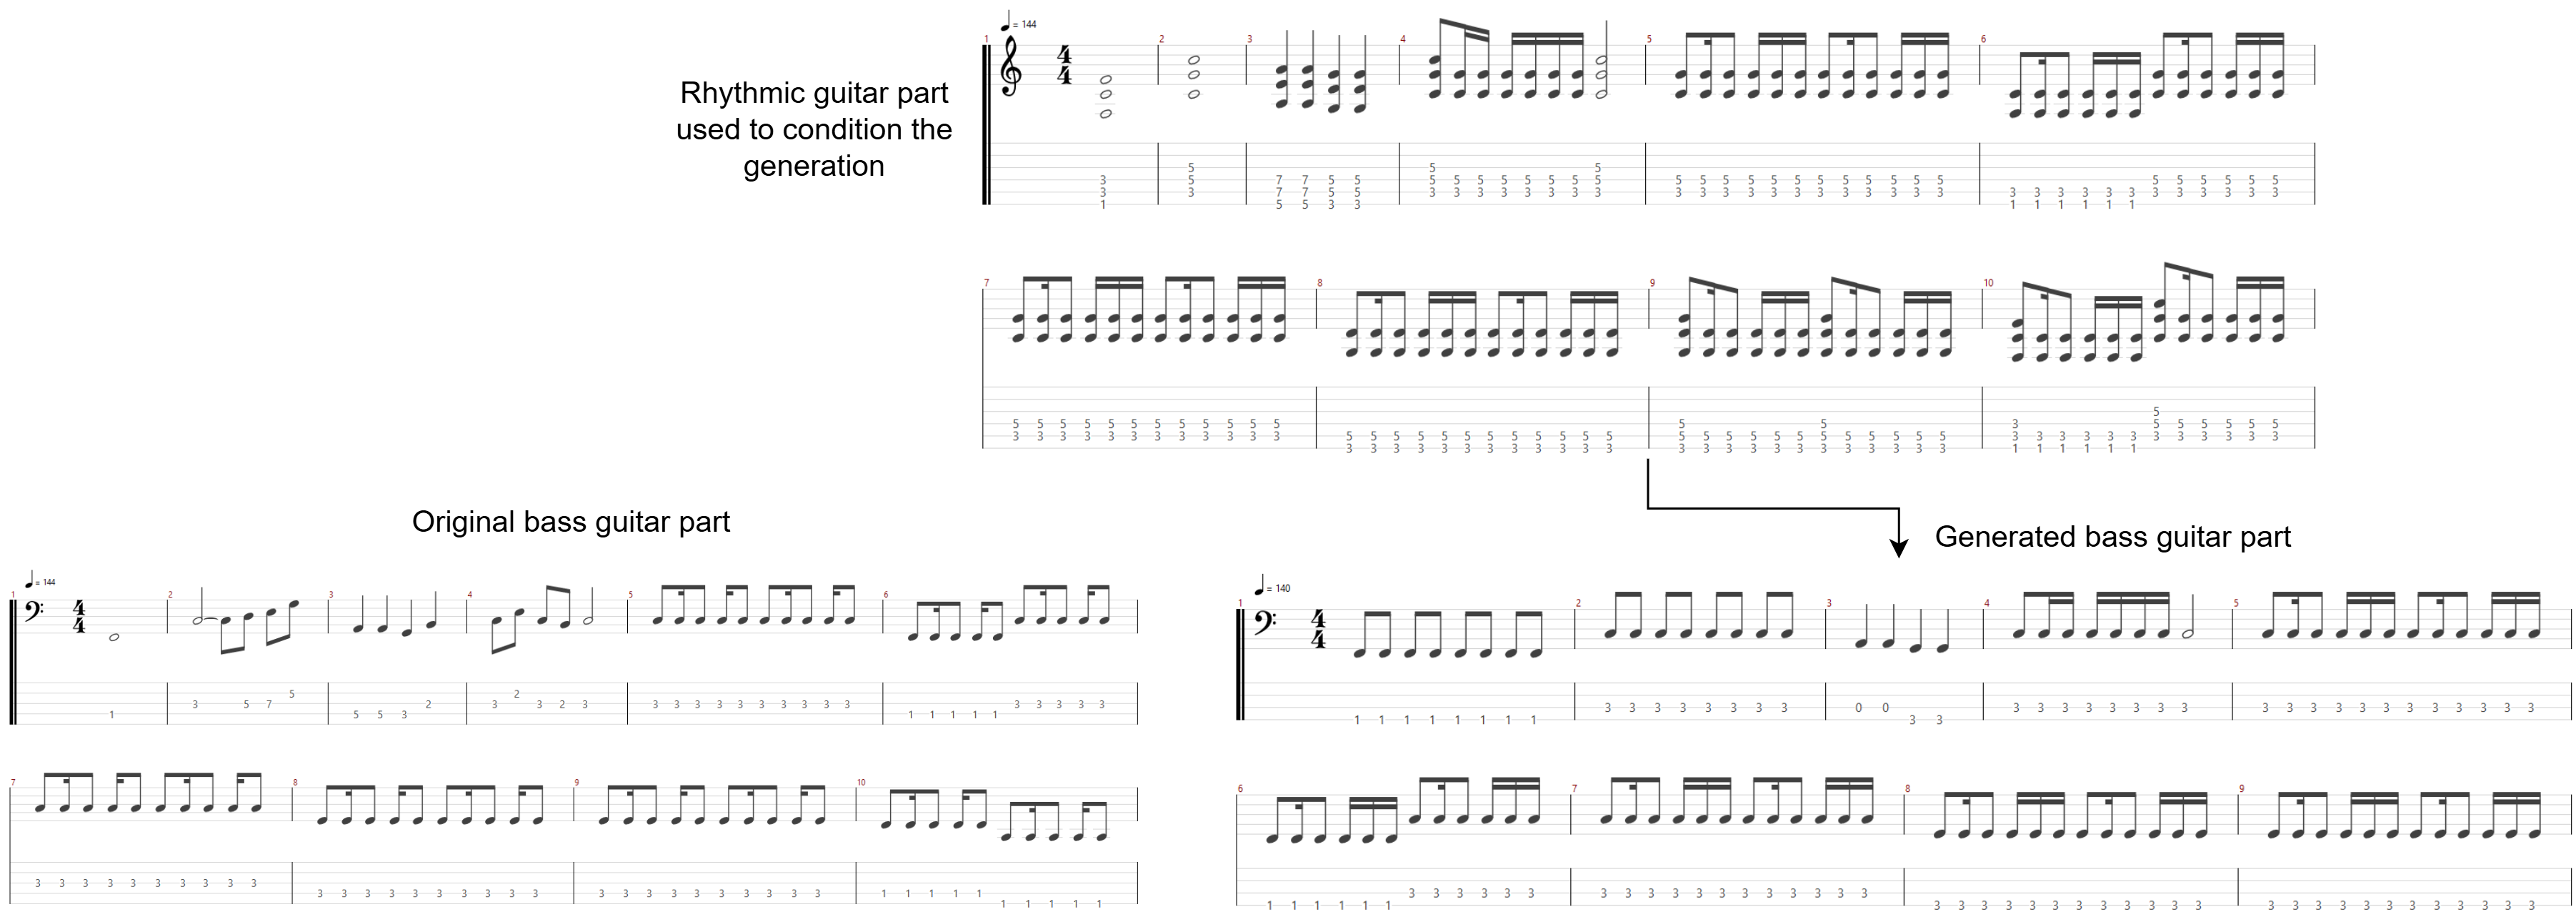
\includegraphics[width=0.9\linewidth]{../images-figures/gen_ricard_peinard.png}
    \caption{Example of 9 measures generated by the model based on the rhythm guitar part of the song "Ricard Peinard" by Ultra Vomit.}
    \label{fig:gen_ricard_peinard}
\end{figure}

Figure \ref{fig:gen_ricard_peinard} shows an excerpt of bass tablatures generated by the model in the metal genre.
Bass guitar in metal music often plays a supportive role, doubling the rhythm guitar part at a lower pitch.
We also display the rhythm guitar part and the original 5-srings bass guitar part.
Several criterion can be qualitatively used to evaluate the model's performance.
First, we can notice that the generated part is harmonically coherent with the rhythm guitar part:
on the first measure the bass plays several F notes, while the rhythm guitar plays a chord composed of F, C and G notes.
Rhythmically, the generated part either copies the rhythm guitar or plays a simpler pattern such as a succession of eighth notes.
This is a correct outcome in the context of metal music, but needs to be further evaluated in other genres.
Finally, one may notice that the generated part is very close to the original bass part on measures 5 to 8.
% FIGURE EXAMPLE 2: INDIE ROCK: ARCTIC MONKEYS DO I WANNA KNOW

\begin{figure}[!ht]
    \centering
    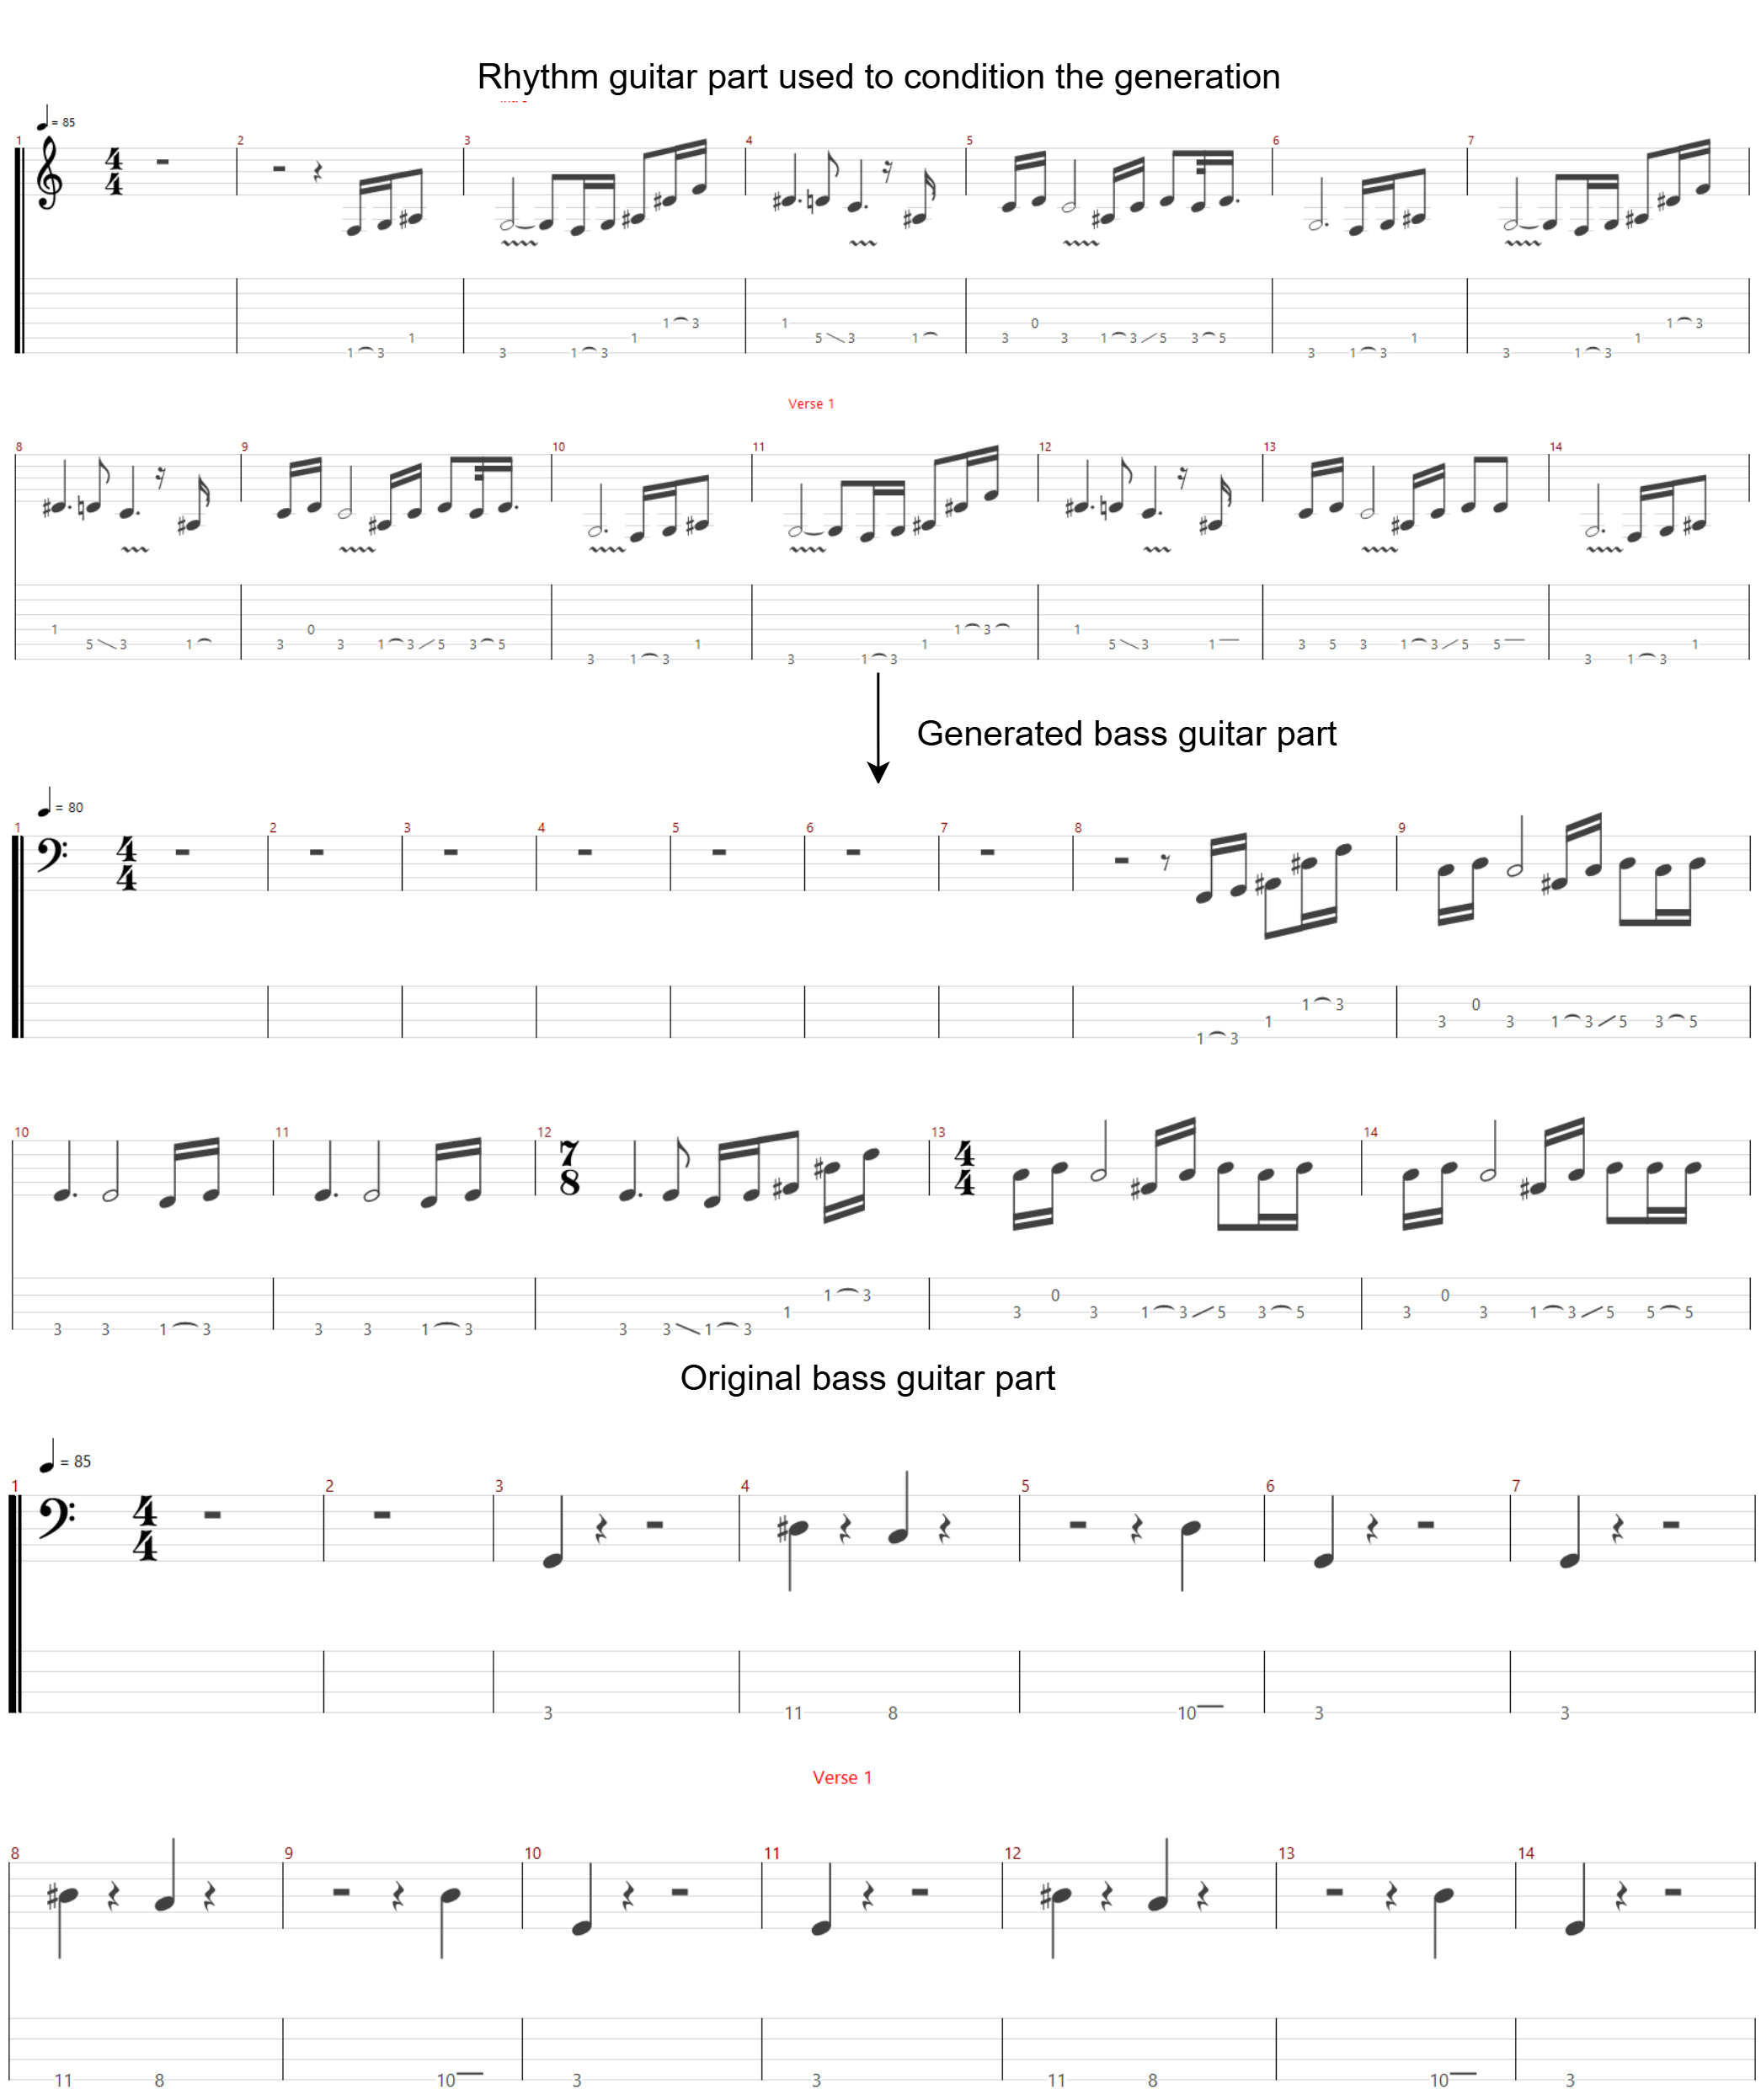
\includegraphics[width=0.85\linewidth]{../images-figures/gen_arctic_monkeys.png}
    \caption{Example of 9 measures generated by the model based on the rhythm guitar part of the song "Do I Wanna Know" by Arctic Monkeys.}
    \label{fig:gen_arctic_monkeys}
\end{figure}

Figure \ref{fig:gen_arctic_monkeys} shows an excerpt of bass tablatures generated by the model in the indie rock genre.
Bass guitar's role in indie rock music is hard to define due to the genre's diversity.
However, this example remains particularly interesting as it demonstrates the model's tendency to copy the rhythm guitar part even when very simple parts would be more appropriate.
Here the original bass part is basic yet essential, providing groove and structure to the song using quarter notes at specific onsets.
Nonetheless, the generated part remains harmonically and rhythmically coherent with the rhythm guitar part.
This example also shows a recurrent issue in the model's inability to follow a time signature.
Here measure 12 becomes a 7/8 instead of a 4/4 (the model forgot an eighth note in the measure).
We could try to handle this issue by adding a loss term that would penalize the model if the time signature is not respected.

% FIGURE EXAMPLE 3: JAZZ FUNK: HERBIE HANCOCK SATURDAY NIGHT

\begin{figure}[!ht]
    \centering
    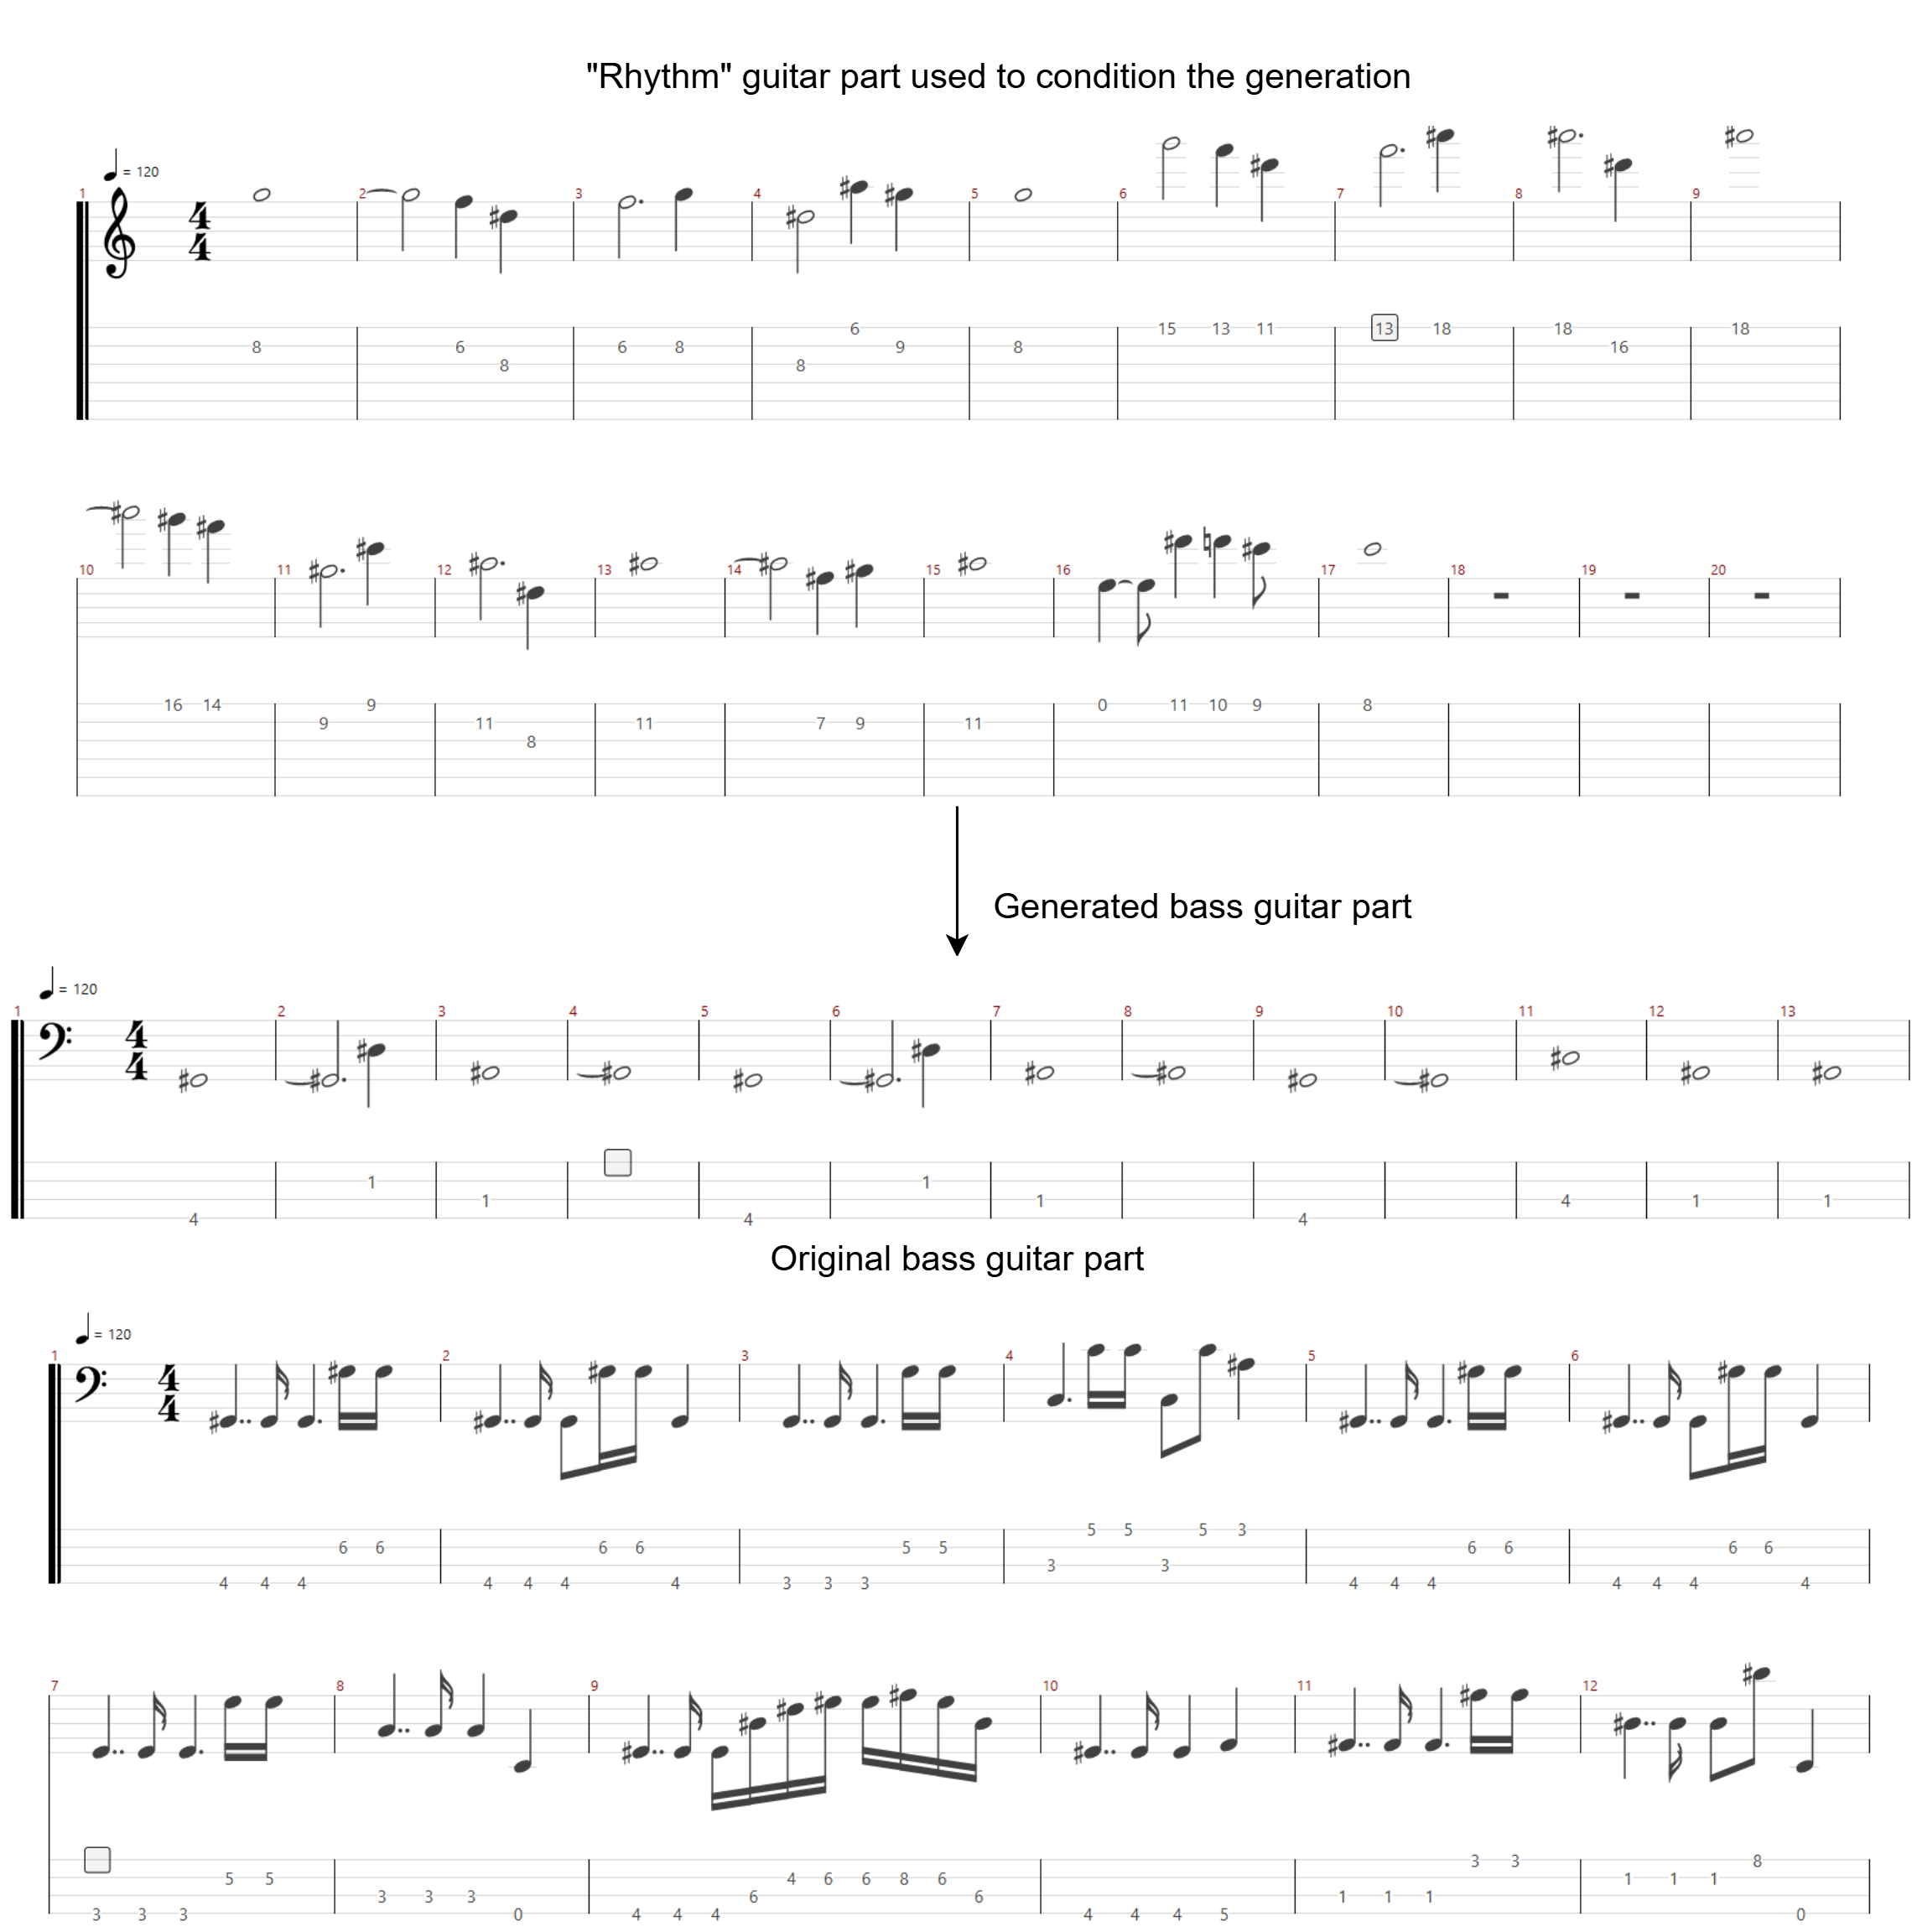
\includegraphics[width=0.9\linewidth]{../images-figures/gen_herbie_hancock.png}
    \caption{Example of 9 measures generated by the model based on the rhythm guitar part of the song "Saturday Night" by Herbie Hancock.}
    \label{fig:gen_herbie_hancock}
\end{figure}

Figure \ref{fig:gen_herbie_hancock} shows an excerpt of bass tablatures generated by the model in the jazz funk genre.
Bass guitar in jazz funk music often plays a more melodic role, with complex rhythmic patterns and harmonies.
Moreover, there are generally no rhythm guitar parts strictly speaking in jazz funk music, so the model generates using a more melodic guitar part.
As expected, the generated part is way simpler than the original bass part.
It is meant to be an accompaniment to the guitar part, not a melodic part.
Moreover, jazz funk music often uses complex harmonies, so the model has a hard time following the harmonic progression.
This genre can be considered as a limit case for the model.
As jazz funk is not significantly represented in the dataset, nad the model was trained on an agglomerate of genres, it is not able to generate coherent bass lines.

To summarize, the model has great potential in generating bass tablatures of accompaniment that are harmonically and rhythmically coherent with the rhythm guitar part.
However, it struggles to adapt to the specificities of each genre and can still make rhythmical mistakes.
We tried to build an adaptable model that could generate bass lines for a wide range of styles,
but it would be interesting to analyze the model's performance on a specific genre if trained on said genre only.

\subsection{Conclusion}  

In this work, we explored the conditional generation of bass guitar tablatures using a transformer-based model trained on the DadaGP dataset.
We implemented a detailed data preprocessing pipeline, including instrument-specific token extraction, rhythm guitar identification, and structured sequence formatting.
Our approach enables the generation of bass lines that are harmonically and rhythmically coherent with a given rhythm guitar part.  
Our results demonstrate that the model effectively captures the structural role of the bass guitar in various genres, successfully aligning with the rhythmic and harmonic elements of the accompaniment.
However, we also identified certain limitations, such as the model's tendency to replicate rhythmic patterns excessively and occasional inconsistencies in time signature adherence.
While our study establishes a strong foundation for conditioned bass tablature generation, further refinements in model design, data representation, and evaluation methods could enhance its practical applicability.
The next section discusses possible improvements and future research directions.

\subsection{Perspectives}

With additional time, several improvements could be made to the model architecture and tuning, data processing, and evaluation.
One potential enhancement is simplifying the model by removing one of the dense layers in the embedding process, which could reduce complexity without significantly impacting performance.
Additionally, experimenting with compound word tokenization as an alternative to the current DadaGP method might yield more meaningful representations.
We saw in the jazz funk example that the model struggles with genres that are not well-represented in the dataset.
Therefore, training the model or fine-tuning it on specific genres could be a good way to both improve the model's performance on that genreand be able to evaluate it more accurately on a more precise task.

We also only used rhythm guitar parts to condition the model, but other instruments could be used as conditioning instruments.
We cited drums as a possible conditioning instrument that lacked harmonic informaton.
However, a combination of drums and rhythm guitar could improve the model's performance, although the encoder sequence length would be greatly increased.
Beyond architectural changes, a user study could be conducted to assess the quality of the generated bass lines, providing valuable insights into the model's musical coherence.
Finally, evaluating the model's environmental impact using Green AI~\cite{schwartz_green_2020} metrics, specifically by measuring the number of floating point operations (FLOPs), would contribute to a better understanding of its computational efficiency.

